\documentclass{beamer}

\usepackage{verbatim}
\usepackage{graphicx}
\usepackage{booktabs}
\usepackage[brazil]{babel}
\usepackage[utf8x]{inputenc}
\usepackage[portuguese, ruled, linesnumbered]{algorithm2e}
\usepackage{float}
\usetheme{Madrid}
\usepackage{tikz}
\usepackage{listings}
\usepackage{adjustbox}
\usepackage{amsmath}
\usepackage{geometry}
\usepackage{colortbl}

\usepackage{tikz}
\usetikzlibrary{positioning}
\usepackage[american]{circuitikz}

\newcommand{\cinza}{\cellcolor[gray]{0.5}}
\definecolor{gray}{gray}{0.6}

\usetikzlibrary{shapes,arrows}


\definecolor{codegreen}{rgb}{0,0.6,0}
\definecolor{codegray}{rgb}{0.5,0.5,0.5}
\definecolor{codepurple}{rgb}{0.58,0,0.82}
\definecolor{backcolour}{rgb}{0.95,0.95,0.92}

\lstdefinestyle{mystyle}{
	frame = tb,
	backgroundcolor=\color{backcolour},   
	commentstyle=\color{codegreen},
	keywordstyle=\color{magenta},
	numberstyle=\tiny\color{gray},
	stringstyle=\color{codepurple},
	basicstyle=\footnotesize,
	breakatwhitespace=false,         
	breaklines=true,                 
	captionpos=b,                    
	keepspaces=false,                 
	numbers=left,                    
	numbersep=3pt,                  
	showspaces=false,                
	showstringspaces=false,
	showtabs=false,                  
	tabsize=2
}

\lstset{style=mystyle}

\title[Aula 02 - Confecção de PCB]{Aula 02 - Do Esquemático à PCB}

\author[CAECP]{Wall Berg M. S. Morais\\Centro Acadêmico de Engenharia de Computação (CAECP)}

\institute[UTFPR] 
{
  Departamento de Informática - DAINF \\
  Universidade Tecnológica Federal do Paraná
}

\date[\today]{Construção de Layout para Placas de Circuito Impresso (PCBs) utilizando KiCad\\\today}

\begin{document}
\begin{frame}
  \titlepage
\end{frame}

\begin{frame}
	\tableofcontents
\end{frame}

\section{Introdução}
\begin{frame}{Introdução}
	\begin{block}{Algoritmo de construção com 7 passos}
		\begin{itemize}
			\item Desenhar o esquemático.
			\item Gerar a sequência de componentes.
			\item ``Compilar'' o esquemático com a Joaninha.
			\pause
			\item Gerar o \textit{Netlist}.
			\item Associar os componentes descritos no \textit{Netlist} à componentes reais.
			\item Fazer o roteamento da PCB.
			\item Imprimir a PCB.
			\pause
			\item \textbf{É UMA RECEITA DE BOLO!!!}
		\end{itemize}
	\end{block}	
\end{frame}

\begin{frame}{Introdução}
	\begin{block}{Estudo com um simples filtro de 2º ordem}
		\begin{itemize}
			\item As imagens dos slides a seguir leva em consideração um filtro de segunda ordem na topologia \textit{Sallen-Key} com \textit{buffer} de entrada e saída. Considerar $C_1 = 10nF$, $C_2 = 20nF$, $R_{1,2} = 120k\Omega$.
		\end{itemize}
	\end{block}

   	\begin{figure}[H]
		\centering
		\resizebox{0.7\columnwidth}{!}{
			\begin{circuitikz}[line width=1pt]
				\draw (0,0) node[op amp,yscale=-1] (opamp) {};
				\node [left=0.8cm of opamp.+] (p1) {};
				\node [left=1.5cm of p1] (p2) {};
				\node [left=1.5cm of p2] (p3) {};
				\node [below=1.5cm of p1] (p4) {};
				\node [left=0.2cm of opamp.-,coordinate] (m1) {};
				\node [above = 1cm of p2] (f1) {};
				\node [right=4cm of f1,coordinate] (f2) {};
				\node [right = 0.5cm of opamp.out,coordinate] (f3) {};
				\node [right=1.0cm of opamp.out] (vo) {};
				\node [right=0.2cm of opamp.out,coordinate] (o1) {};
				\node [below=1.2cm of o1,coordinate] (o2) {};
				%%% Draw connections
				\draw (p4) node[ground] {} to[C=$C_2$] (p1) to[short] (opamp.+);
				\draw (p3) node[left] {$v_{in}$} to[R=$R_1$,o-] (p2)
				to[R=$R_2$,*-*] (p1);
				\draw (p2) to[short] (f1) to[C=$C_1$] (f2) -| (f3)
				node[circle,fill=black,scale=0.3,draw] {};
				\draw (opamp.out) to[short,-o] (vo) node[right] {$v_{out}$};
				\draw (opamp.-) to[short] (m1) |- (o2)  to[short,-*] (o1);
			\end{circuitikz}
		}
		\caption{\textit{Sallen-Key} Passa Baixas}
		\label{sallen-key}
	\end{figure}
\end{frame}

\begin{frame}{Introdução}
	\begin{block}{Validação de Aprendizado - Projeto Final}
		\begin{itemize}
			\item Confecção de PCB para um conversor CC/CC abaixador de tensão, o \textit{Buck}.
		\end{itemize}
	\end{block}
	\begin{figure}[H]
		\centering
		\resizebox{0.9\columnwidth}{!}{
			\begin{circuitikz}
				\draw
				(0, 0)
				to[battery1, v_=$V_{in}$] ++(0, -3) coordinate (nodecommon)
				(2, 0)
				node[nigfete, bodydiode, rotate=90] (fet) {}
				(fet.D)
				to[short] (0, 0)
				(fet.G)
				to[short] ++(0, -0.1)
				node[right] {} ++(0, -0.25) node[draw] {Driver}
				(nodecommon)
				to[short] ++(3.5, 0)
				to[D, l_=$D$] ++(0, 3)
				|- (fet.S)
				(fet.S)
				to[short] ++(1, 0)
				to[L, l_=$L$] ++(3, 0) coordinate (node1)
				to[C, l_=$C$] ++(0, -3)
				-| (nodecommon)
				(node1)
				to[short] ++(2, 0)
				to[R, l_=$R_L$] ++(0, -3)
				to[short] (nodecommon)
				(fet.S)
				to[short] ++(0, -0.1)
				node[sground, yscale=0.5, xscale=0.5] {}
				(node1)
				to[short, -o] ++(4, 0) coordinate (out+)
				(nodecommon)
				to[short, -o] ++(10.75, 0) coordinate (out-)
				(out+)
				to[open, v_=$V_{out}$] (out-)
				(nodecommon)
				-| ++(5.5, -0.1)
				node[ground] {}
				;
			\end{circuitikz}
		}
		\caption{Conversor CC-CC abaixador de tensão - Buck.}
		\label{fig:buck}
	\end{figure}
\end{frame}

\section{Desenhando o Esquemático}
\begin{frame}{Desenhando o Esquemático}
	\begin{itemize}
		\item Tela inicial do esquemático.
	\end{itemize}
	\begin{figure}
		\centering
		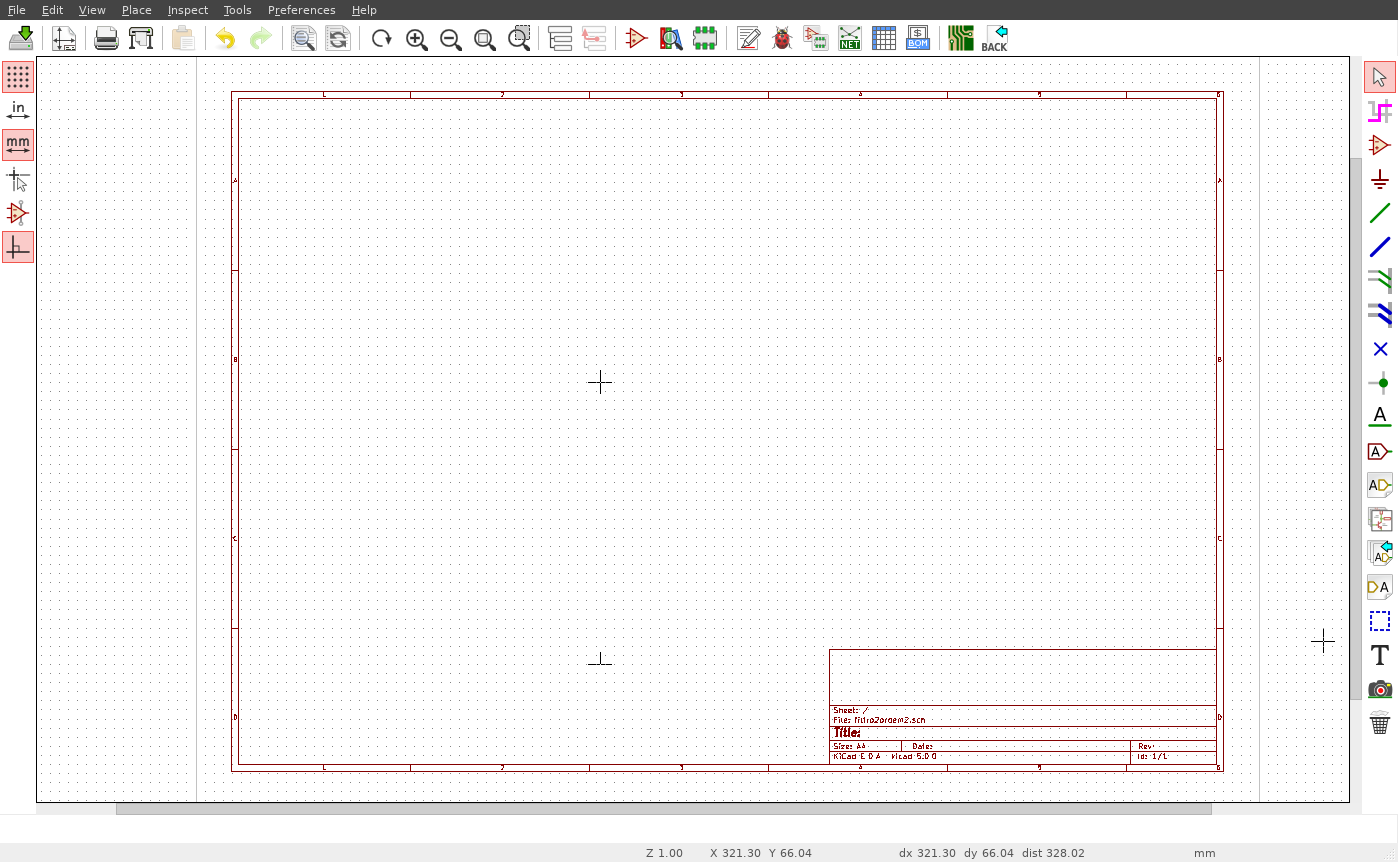
\includegraphics[width=0.8\textwidth]{Imagens/00_pagina_esquematico.png}
		\caption{Tela Inicial do Esquemático}
	\end{figure}
\end{frame}

\begin{frame}{Desenhando o Esquemático}
	\begin{block}{Atalhos mais utilizados}
		\begin{itemize}
			\item \texttt{A} - Adicionar Componente.
			\item \texttt{W} - Desenhar Fio.
			\item \texttt{M} - Mover Componente.
			\item \texttt{R} - Rotacionar.
			\item \texttt{Q} - Marcar pino como não conectado.
			\item \texttt{Del} - Deletar Componente.
			\item \texttt{Ctrl + C} - Copia.
			\item \texttt{Ctrl + Alt + H} - Adicionar \textit{label} global.
		\end{itemize}
	\end{block}
	\pause
	\begin{block}{Atalhos de Componentes}
		\begin{itemize}
			\item \texttt{V} - Definir Valor
			\item \texttt{E} - Editar Componente -- \textbf{Olhar \textit{datasheet} de componente}.
			\item \texttt{C} - Duplicar
		\end{itemize}
	\end{block}
\end{frame}

\begin{frame}{Adicionar Componente}
	\begin{block}{Atalho}
		\begin{itemize}
			\item \texttt{A} - Adicionar Componente.
		\end{itemize}
	\end{block}
	\begin{figure}
		\centering
		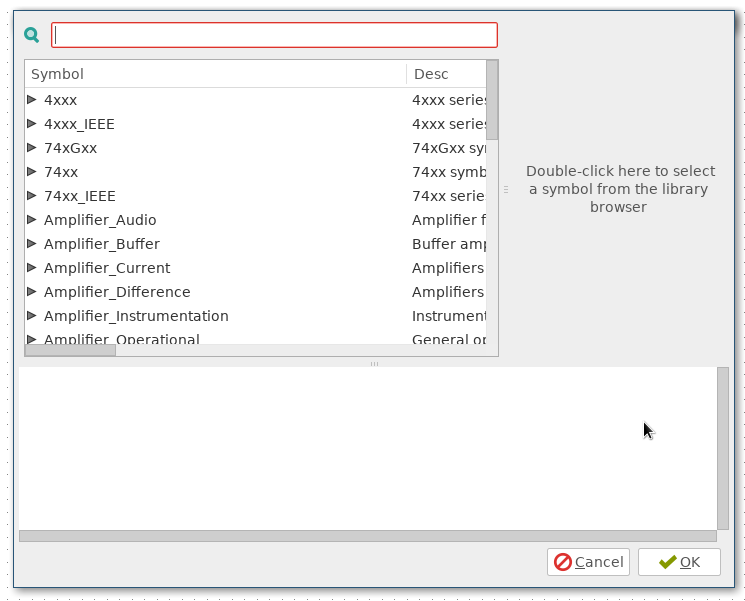
\includegraphics[width=0.55\textwidth]{Imagens/01_adicionar_componente.png}
		\caption{Janela para adicionar componentes.}
	\end{figure}
\end{frame}

\begin{frame}{Editar Componente - Ver \textit{datasheet}}
	\begin{block}{Atalho}
		\begin{itemize}
			\item \texttt{E} - Editar Componente
		\end{itemize}
	\end{block}
	\begin{figure}
		\centering
		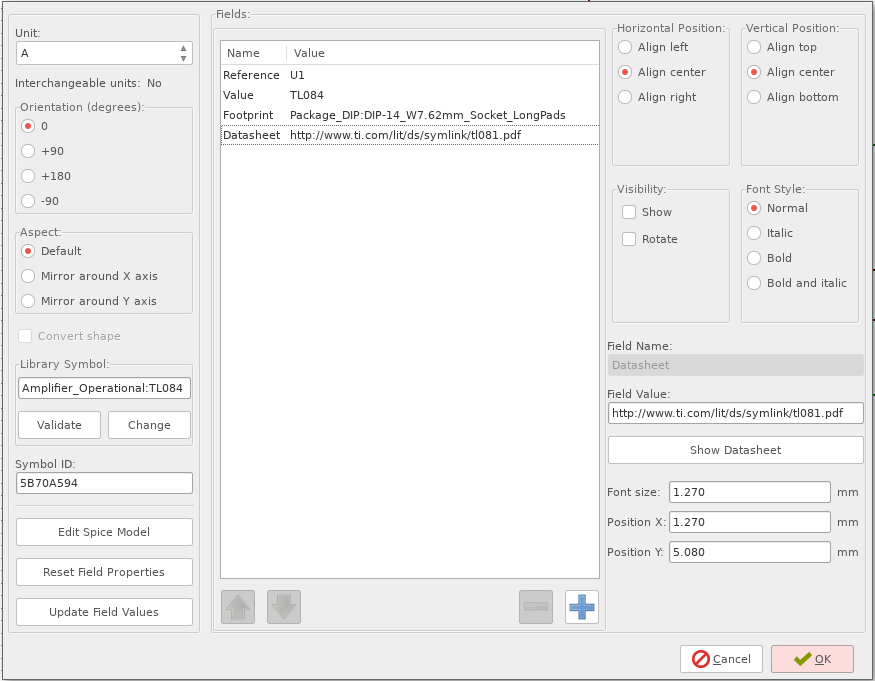
\includegraphics[width=0.55\textwidth]{Imagens/1_1_editar_componente_datasheed.png}
		\caption{Janela para editar componente.}
	\end{figure}
\end{frame}

\begin{frame}{Circuito do Filtro}{Pré-Montagem}
	\begin{figure}
		\centering
		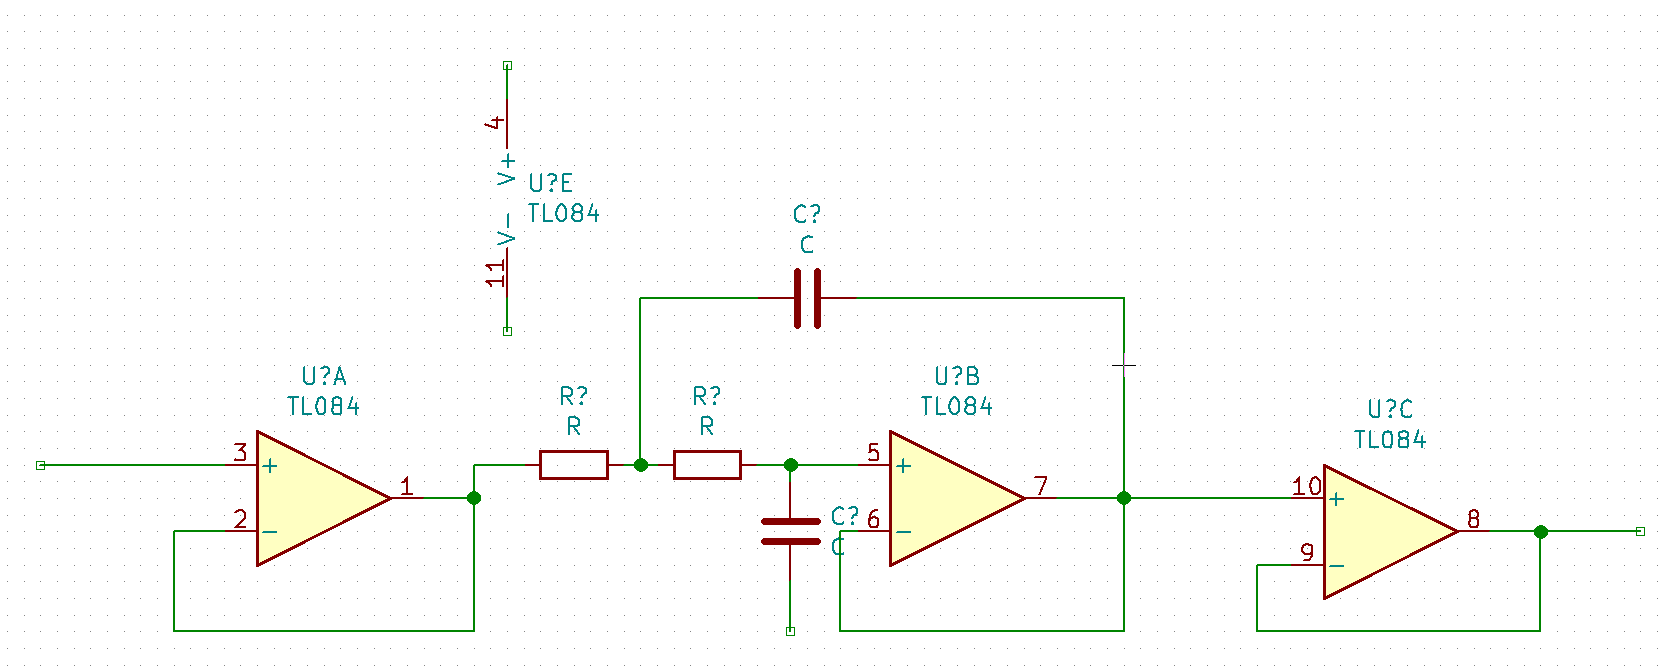
\includegraphics[width=1\textwidth]{Imagens/02_circuito_filtro_pre_montado.png}
		\caption{Filtro Pré-Montado}
	\end{figure}
\end{frame}

\begin{frame}{Adicionando \textit{Labels}}
	\begin{block}{Atalho}
		\begin{itemize}
			\item \texttt{Ctrl + Alt + H} - Adicionar \textit{label} global.
		\end{itemize}
	\end{block}
	\begin{figure}
		\centering
		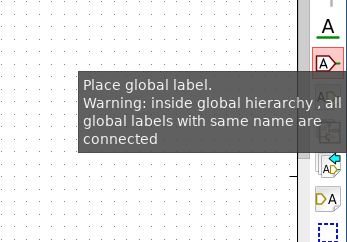
\includegraphics[width=0.6\textwidth]{Imagens/03_label.png}
		\caption{Ícone para adicionar \textit{label}.}
	\end{figure}
\end{frame}

\begin{frame}{Circuito com as \textit{labels} adicionadas}
	\begin{figure}
		\centering
		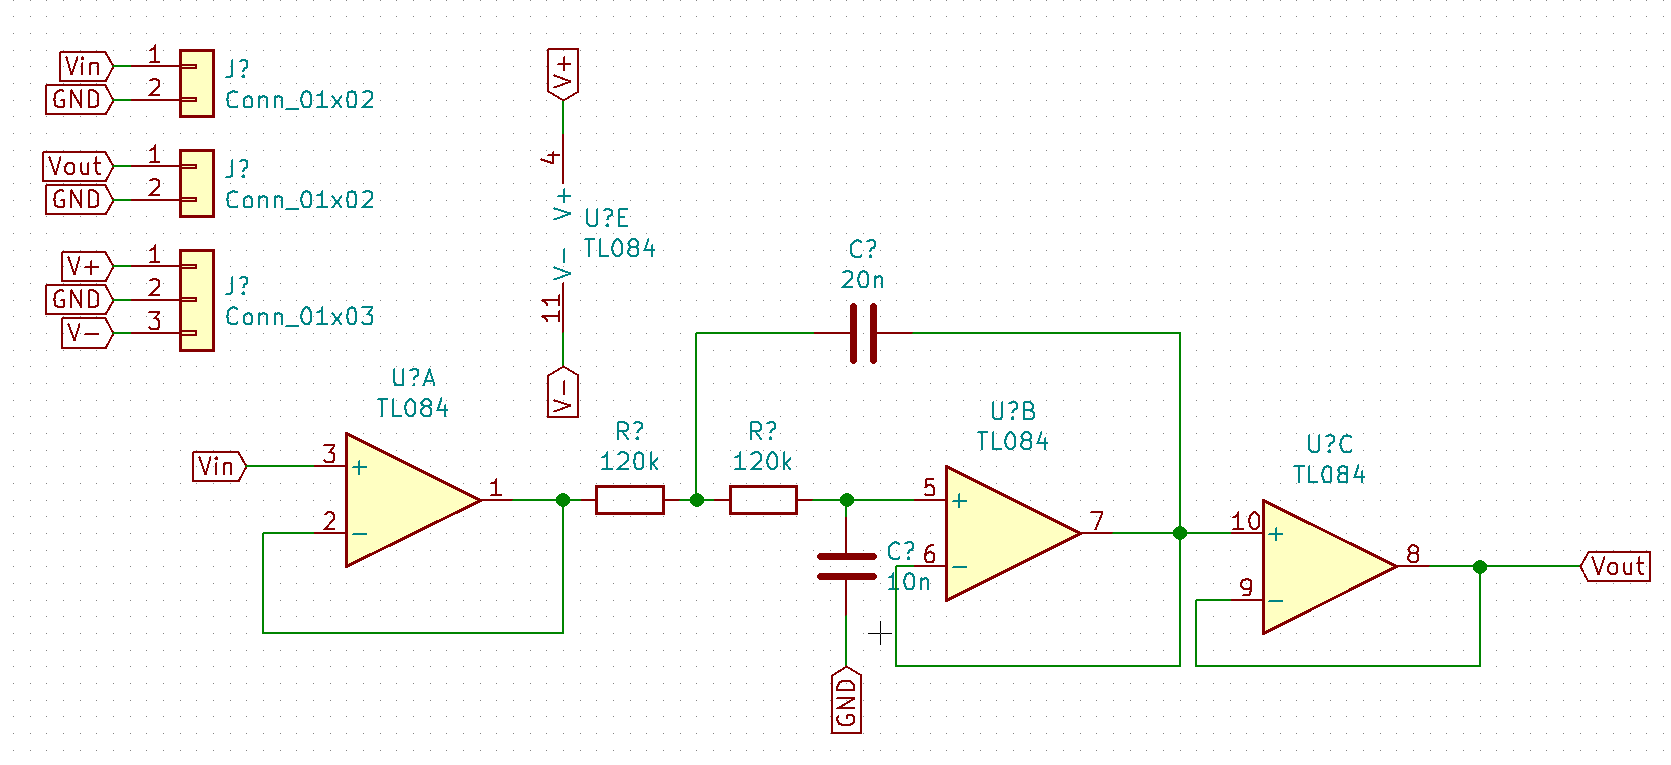
\includegraphics[width=1\textwidth]{Imagens/04_circ_com_label.png}
		\caption{Circuito do filtro com \textit{labels} e conectores.}
	\end{figure}
\end{frame}

\section{\textit{Annotate} - Gerando sequência de componentes}
\begin{frame}{\textit{Annotate} - Gerando sequência de componentes}
	\begin{block}{Pra que serve?}
		\begin{itemize}
			\item Gerar contagem dos componentes.
			\item Sem ele, não é possível ``compilar'' o circuíto.
		\end{itemize}
	\end{block}
	\begin{figure}
		\centering
		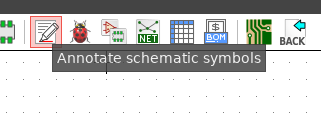
\includegraphics[width=1.0\textwidth]{Imagens/05_anotate_local.png}
		\caption{Localização da opção \textit{annotate} na barra de menu.}
	\end{figure}
\end{frame}

\begin{frame}{\textit{Annotate} - Gerando sequência de componentes}
	\begin{figure}
		\centering
		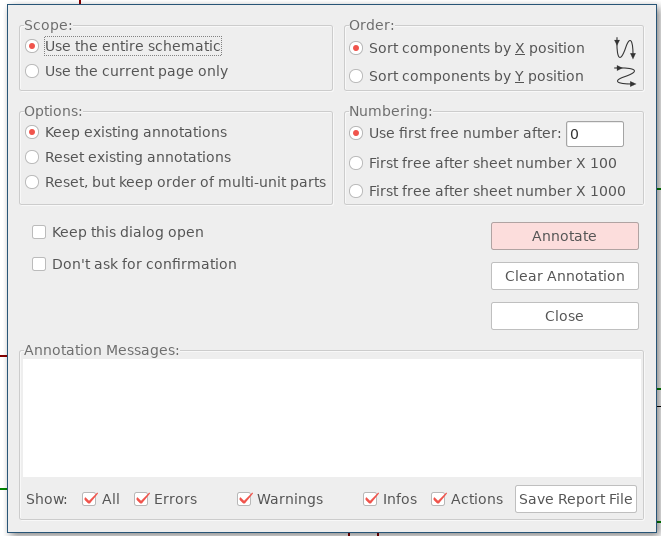
\includegraphics[width=0.7\textwidth]{Imagens/06_anotate_janela.png}
		\caption{Janela que gera as ``anotações'' }
	\end{figure}
\end{frame}

\begin{frame}{\textit{Annotate} - Gerando sequência de componentes}
	\begin{figure}
		\centering
		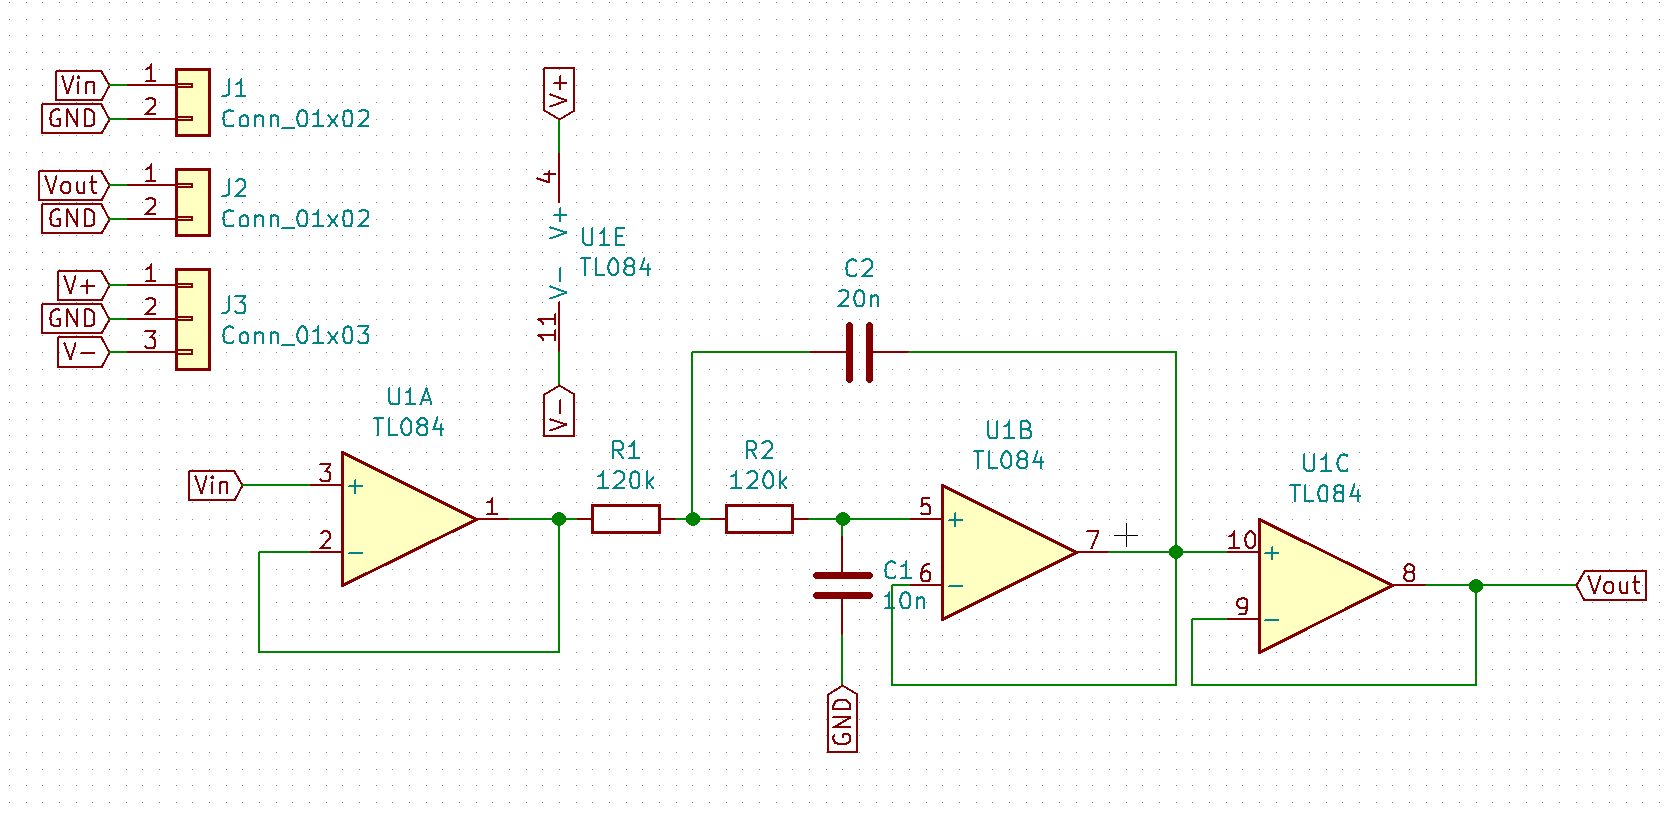
\includegraphics[width=0.95\textwidth]{Imagens/07_circ_com_anotate.png}
		\caption{Circuito com o \textit{annotate}.}
	\end{figure}
	\pause
	\begin{itemize}
		\item O \textit{annotate} muda apenas aquele $?$ nas \textit{``labels''} dos componentes.
	\end{itemize}
\end{frame}

\section{``Compilando'' o esquemático com a Joaninha.}
\begin{frame}{``Compilando'' o esquemático com a Joaninha}
	\begin{block}{Pra que serve?}
		\begin{itemize}
			\item Verificação de erros no circuito.
			\begin{itemize}
				\item Verifica se existe algum componente sem está conectado.
				\item Seu uso não é obrigatório, porém é uma garantia de dizer que o circuito está tudo certo.
			\end{itemize}
		\end{itemize}
	\end{block}
	\begin{figure}
		\centering
		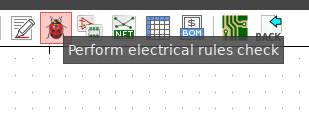
\includegraphics[width=0.8\textwidth]{Imagens/08_joaninha.png}
		\caption{Localização da opção \textit{rules check}(ou joaninha) na barra de menu.}
	\end{figure}
\end{frame}

\begin{frame}{``Compilando'' o esquemático com a Joaninha}
	\begin{figure}
		\centering
		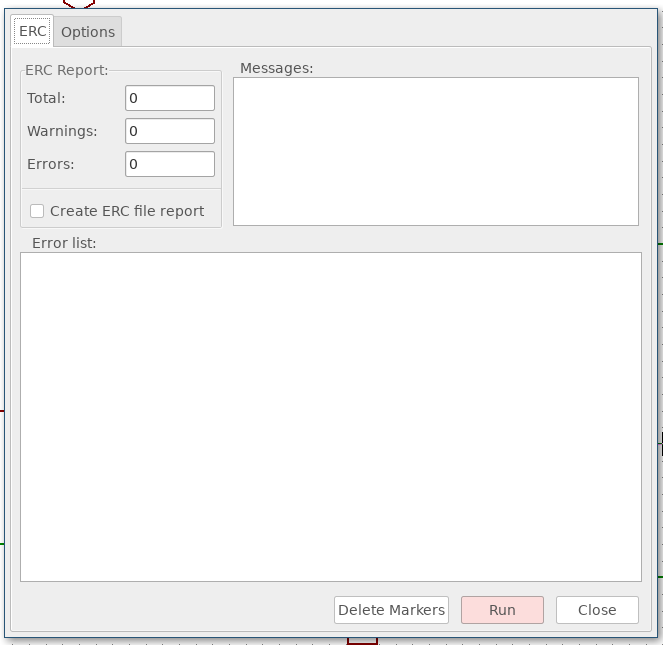
\includegraphics[width=0.5\textwidth]{Imagens/09_joaninha_janela.png}
		\caption{Janela que ``compila'' o circuíto.}
	\end{figure}
	\pause
	\begin{itemize}
		\item É preciso só apertar o botão "Run".
	\end{itemize}
\end{frame}

\begin{frame}{``Compilando'' o esquemático com a Joaninha}
	\begin{figure}
		\centering
		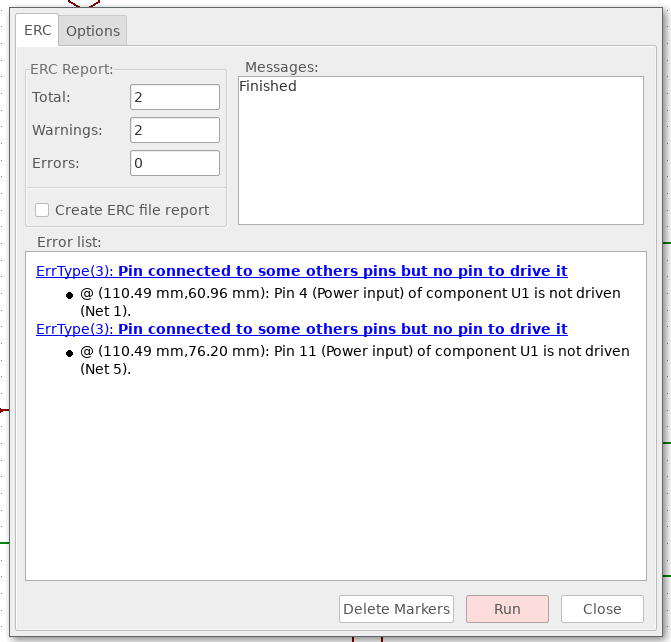
\includegraphics[width=0.6\textwidth]{Imagens/10_joaninha_erro.png}
		\caption{Erro após compilar o circuito anterior.}
	\end{figure}
\end{frame}

\begin{frame}{Indicação de erro gerado pela Joaninha}
	\begin{figure}
		\centering
		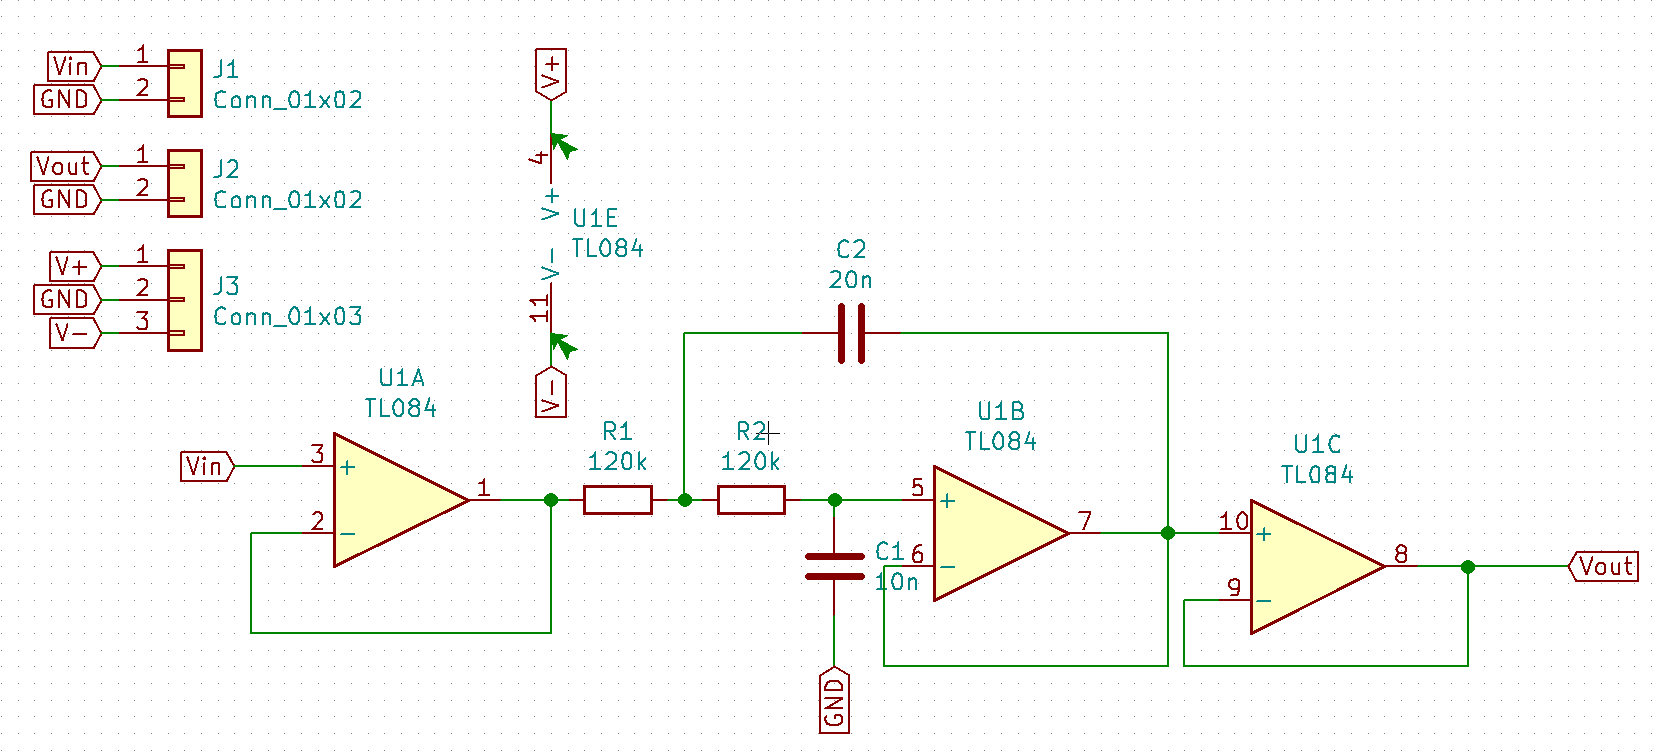
\includegraphics[width=0.9\textwidth]{Imagens/11_erro_no_circuito.png}
		\caption{Erro indicado no circuito pela Joaninha.}
	\end{figure}
	\pause
	\begin{itemize}
		\item A solução é utilizar \texttt{PWR\_FLAG}.
	\end{itemize}
\end{frame}

\begin{frame}{Adicionando \texttt{PWR\_FLAG}}
	\begin{figure}
		\centering
		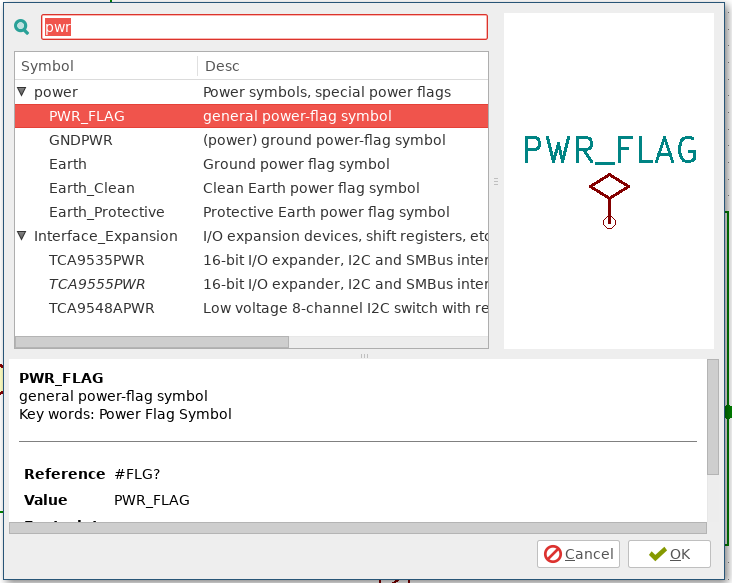
\includegraphics[width=0.7\textwidth]{Imagens/12_add_pwr_flag.png}
		\caption{Janela para adicionar \texttt{PWR\_FLAG}}
	\end{figure}
\end{frame}

\begin{frame}{Adicionando \texttt{PWR\_FLAG}}
	\begin{figure}
		\centering
		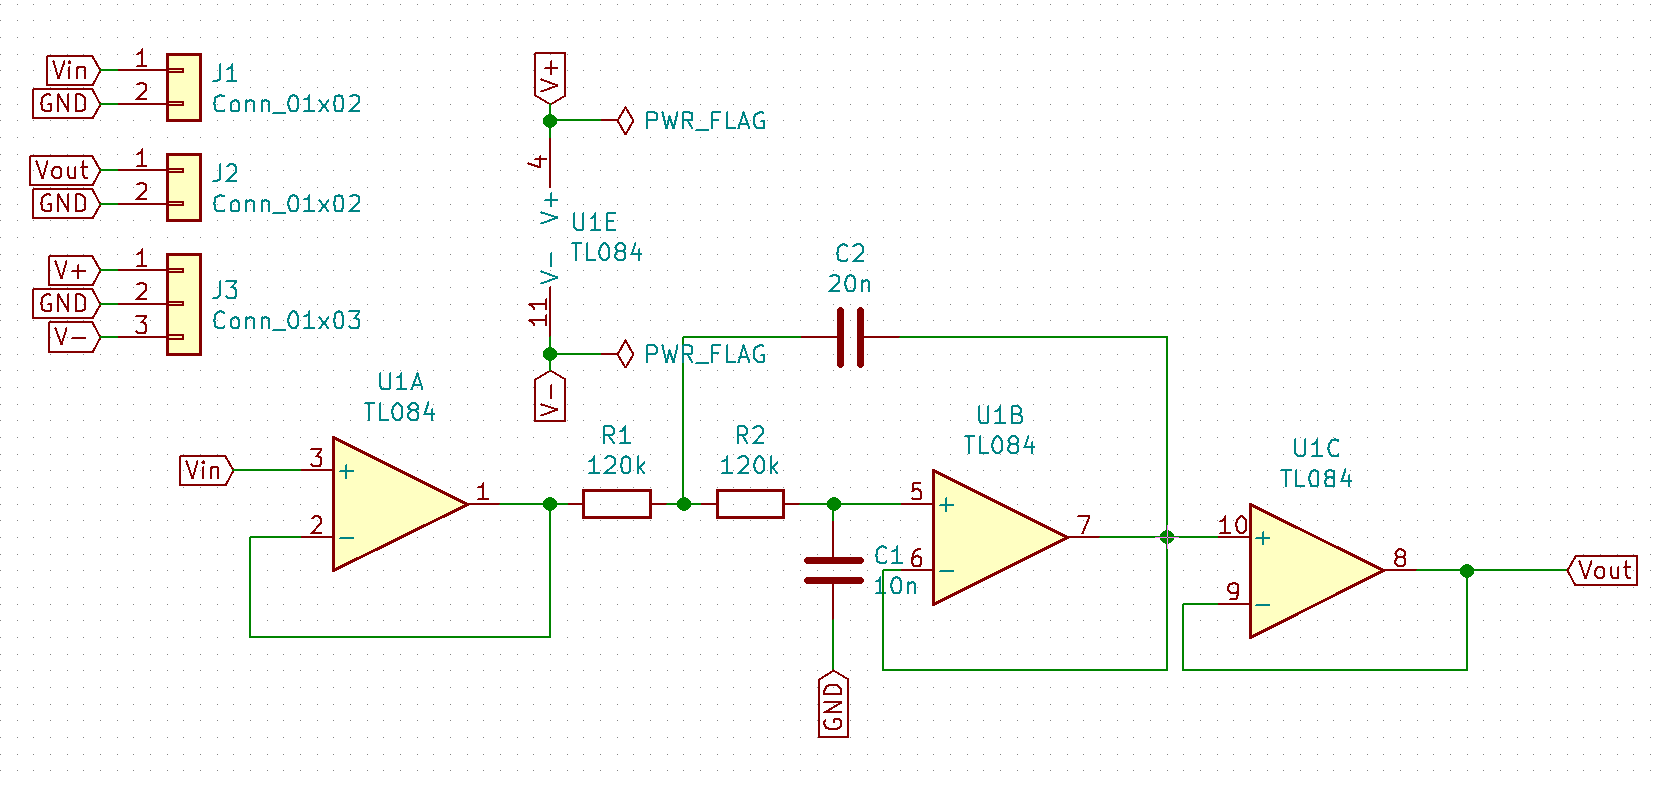
\includegraphics[width=1.0\textwidth]{Imagens/13_circ_com_pwr_flag.png}
		\caption{Circuito com \texttt{PWR\_FLAG}}
	\end{figure}
\end{frame}

\begin{frame}{Verificando novamente o circuito com a Joaninha - Tudo ok}
	\begin{figure}
		\centering
		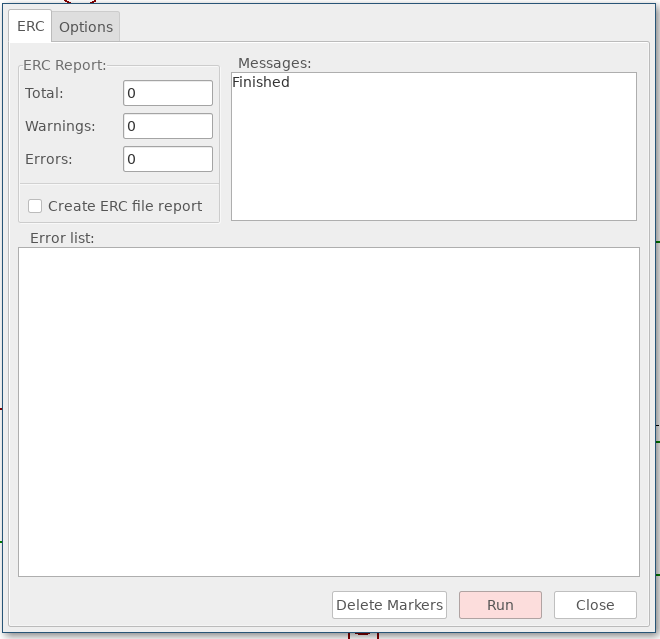
\includegraphics[width=0.55\textwidth]{Imagens/14_joaninha_sem_erro.png}
		\caption{Verificação de circuito sem erros.}
	\end{figure}
\end{frame}

\section{Gerando o \textit{Netlist}}
\begin{frame}{Gerando o \textit{Netlist}}
	\begin{block}{O que é?}
		\begin{itemize}
			\item É um descritor do circuito e seus componentes.
		\end{itemize}
	\end{block}
	\begin{figure}
		\centering
		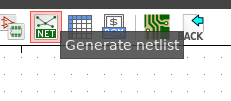
\includegraphics[width=0.8\textwidth]{Imagens/15_netlist.png}
		\caption{Localização da opção para gerar o \textit{netlist}}
	\end{figure}
\end{frame}

\begin{frame}{Gerando o \textit{Netlist}}
	\begin{figure}
		\centering
		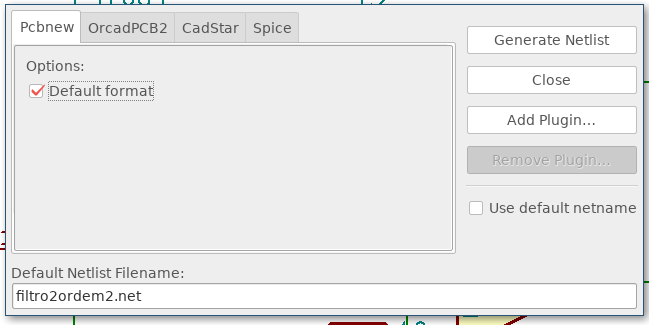
\includegraphics[width=0.8\textwidth]{Imagens/15_netlist_janela.png}
		\caption{Janela para gerar o \textit{netlist}.}
	\end{figure}
	\pause
	\begin{itemize}
		\item Só é necessário apertar no botão para gerar o \textit{netlist}.
		\item Escolher um local para salva-lo.
		\item Recomenda-se colocar na mesma pasta do projeto.
	\end{itemize}
\end{frame}

\section{Associando os componentes descritos no \textit{Netlist} à componentes reais.}
\begin{frame}{Associando os componentes do \textit{netlist} à \textit{footprints}}
	\begin{block}{Pra que serve?}
		\begin{itemize}
			\item É necessário pois são os componentes físicos que estarão na PCB.
			\item É sempre bom tomar cuidado com o tamanho dos componentes escolhidos.
		\end{itemize}
	\end{block}
	\pause
	\begin{figure}
		\centering
		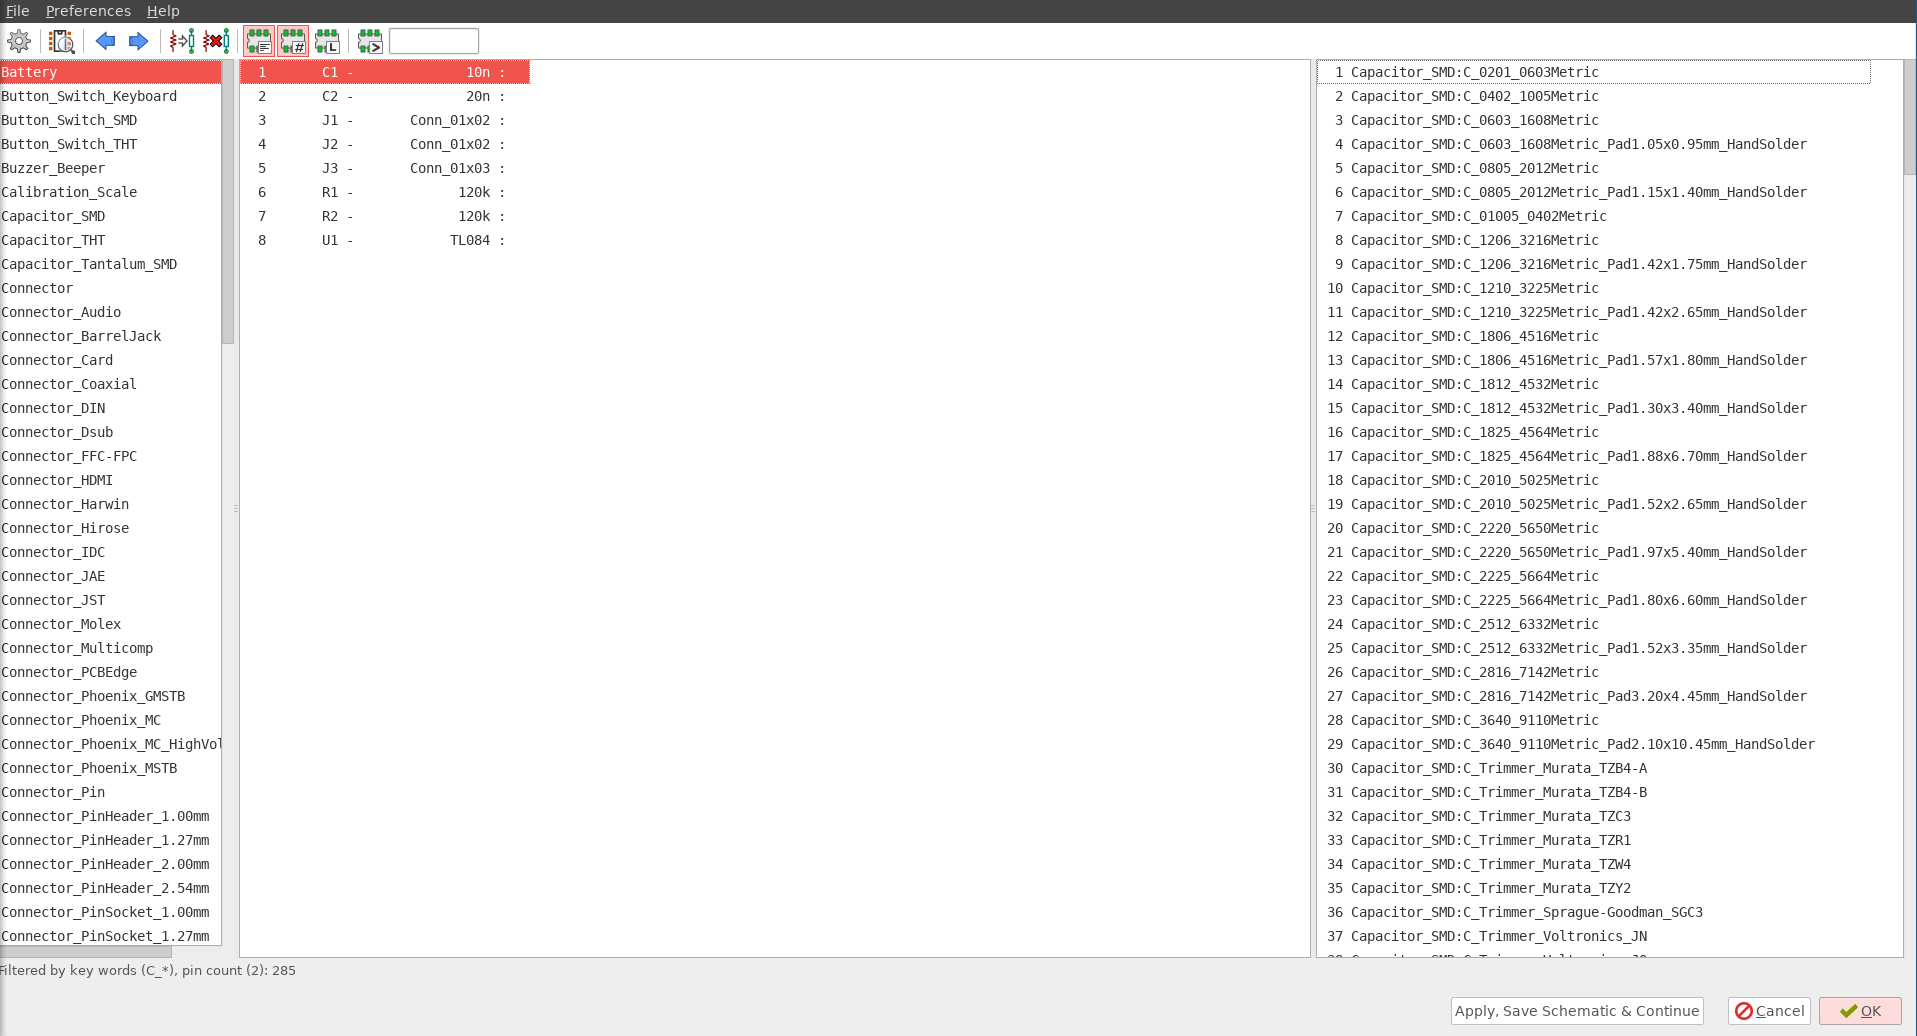
\includegraphics[width=0.65\textwidth]{Imagens/17_associar_janela.png}
		\caption{Janela para escolha de componentes.}
	\end{figure}
\end{frame}

\begin{frame}{Visualizando um \textit{footprint}}
	\begin{block}{Por que?}
		\begin{itemize}
			\item Serve para olhar o componente selecionado no lado direito da tela.
			\item Fazer a escolha certo do mesmo.
		\end{itemize}
	\end{block}
	\pause
	\begin{figure}
		\centering
		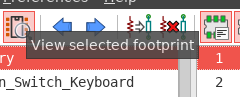
\includegraphics[width=0.8\textwidth]{Imagens/18_ver_componente.png}
		\caption{Localização no menu superior para olhar o \textit{footprint};}
	\end{figure}
\end{frame}

\begin{frame}{Visualizando um \textit{footprint}}
	\begin{figure}
		\centering
		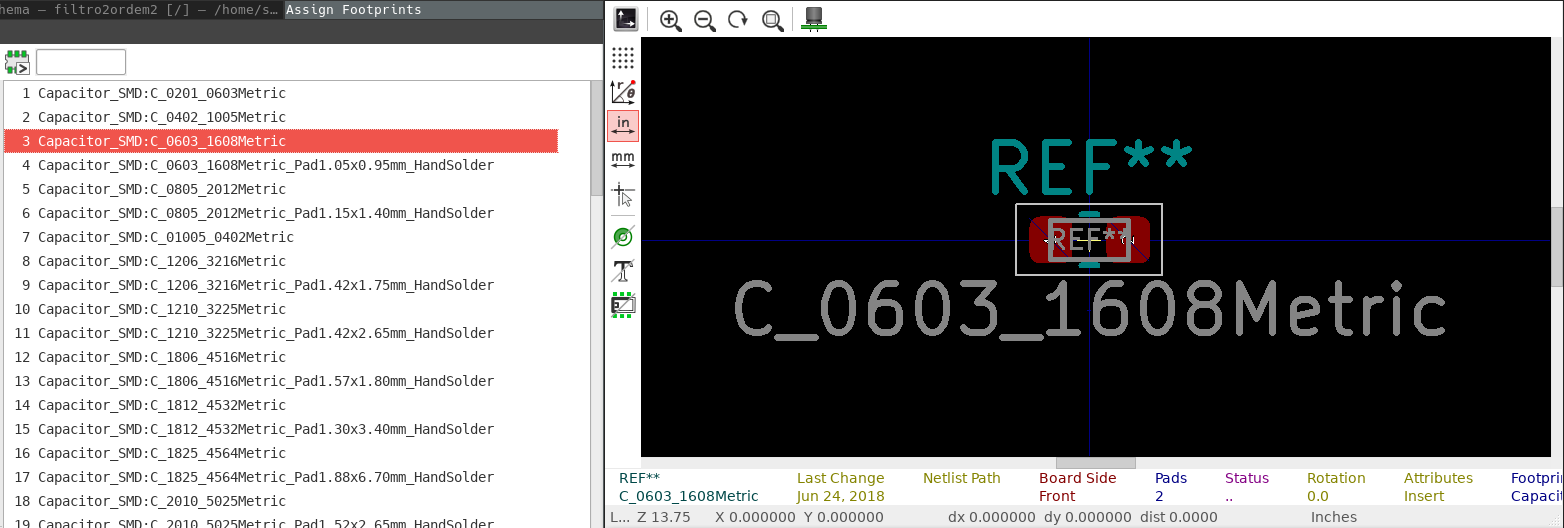
\includegraphics[width=1\textwidth]{Imagens/19_janela_ver_componente.png}
		\caption{Janela de exibição de componente.}
	\end{figure}
	\pause
	\begin{itemize}
		\item Para visualização 3D, ícone no canto esquerdo.
	\end{itemize}
\end{frame}

\begin{frame}{Visualizando um \textit{footprint} em 3D}
	\begin{figure}
		\centering
		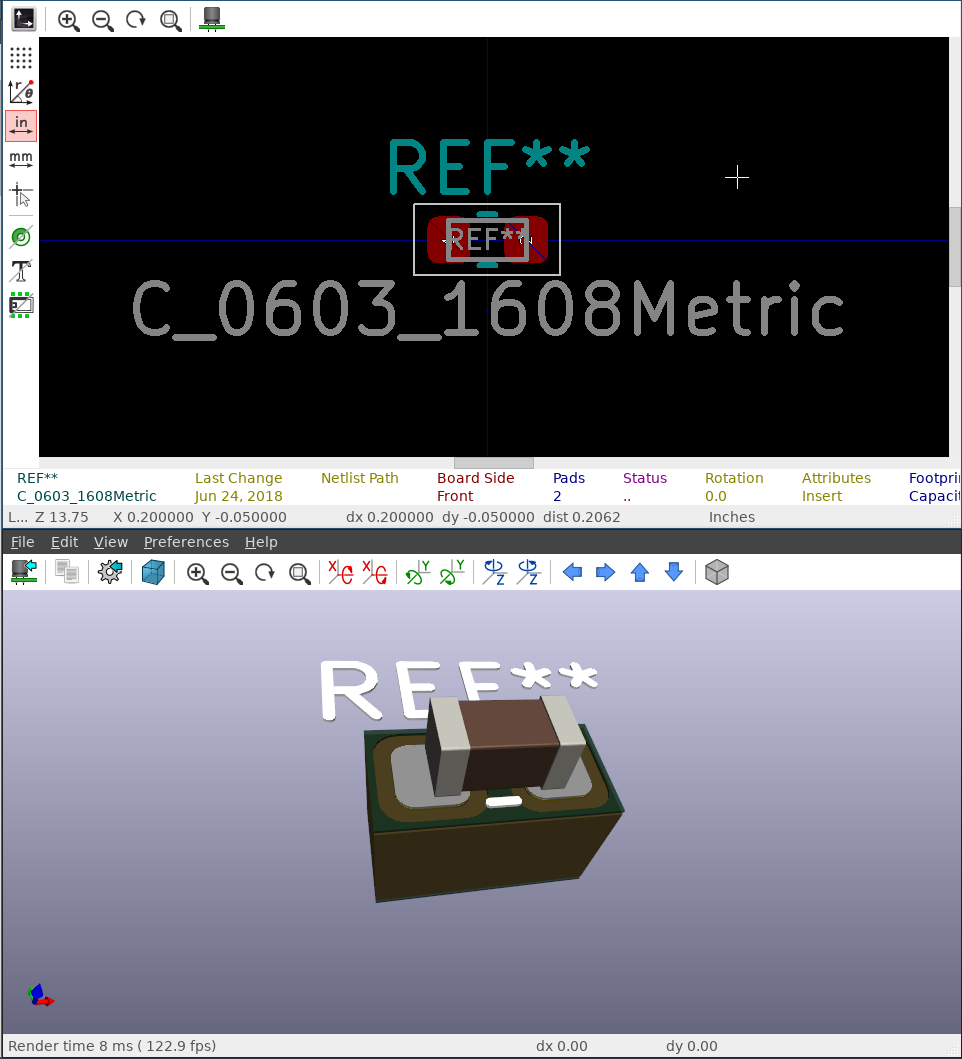
\includegraphics[width=0.4\textwidth]{Imagens/21_view_3d_janela.png}
		\caption{Visualização em 3D de um capacitor SMD.}
	\end{figure}
	\pause
	\begin{itemize}
		\item \textbf{Essa visualização 3D não funciona para todos os componentes.}
	\end{itemize}
\end{frame}

\begin{frame}{Medindo distancia entre pinos de componentes}
	\begin{block}{Pra que serve?}
		\begin{itemize}
			\item Pra ter noção do tamanho de um componente e distância entre os pinos.			
		\end{itemize}
	\end{block}
	\pause
	\begin{figure}
		\centering
		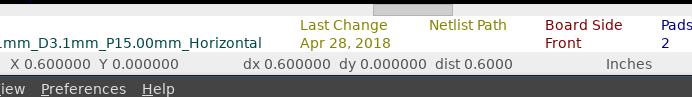
\includegraphics[width=1\textwidth]{Imagens/22_medindo_distancias.png}
		\caption{Barra com local do cursor sobre o \textit{footprint} e um $dx$ e $dy$.}
	\end{figure}
	\pause
	\begin{block}{Atalho}
		\begin{itemize}
			\item \texttt{Espaço} - Zerar a contagem de $dx$ e $dy$.
		\end{itemize}
	\end{block}
\end{frame}

\begin{frame}{Medida de distância}
	\begin{block}{Cuidado}
		\begin{itemize}
			\item Conferir a unidade de medida selecionada e colocar para $mm$.
		\end{itemize}
	\end{block}
	\begin{figure}
		\centering
		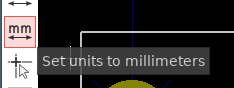
\includegraphics[width=1\textwidth]{Imagens/22_cuidado_unidade.png}
		\caption{Menu lateral para escolha das unidade de medida.}
	\end{figure}
\end{frame}

\begin{frame}{Terminando de associar os componentes}
	\begin{figure}
		\centering
		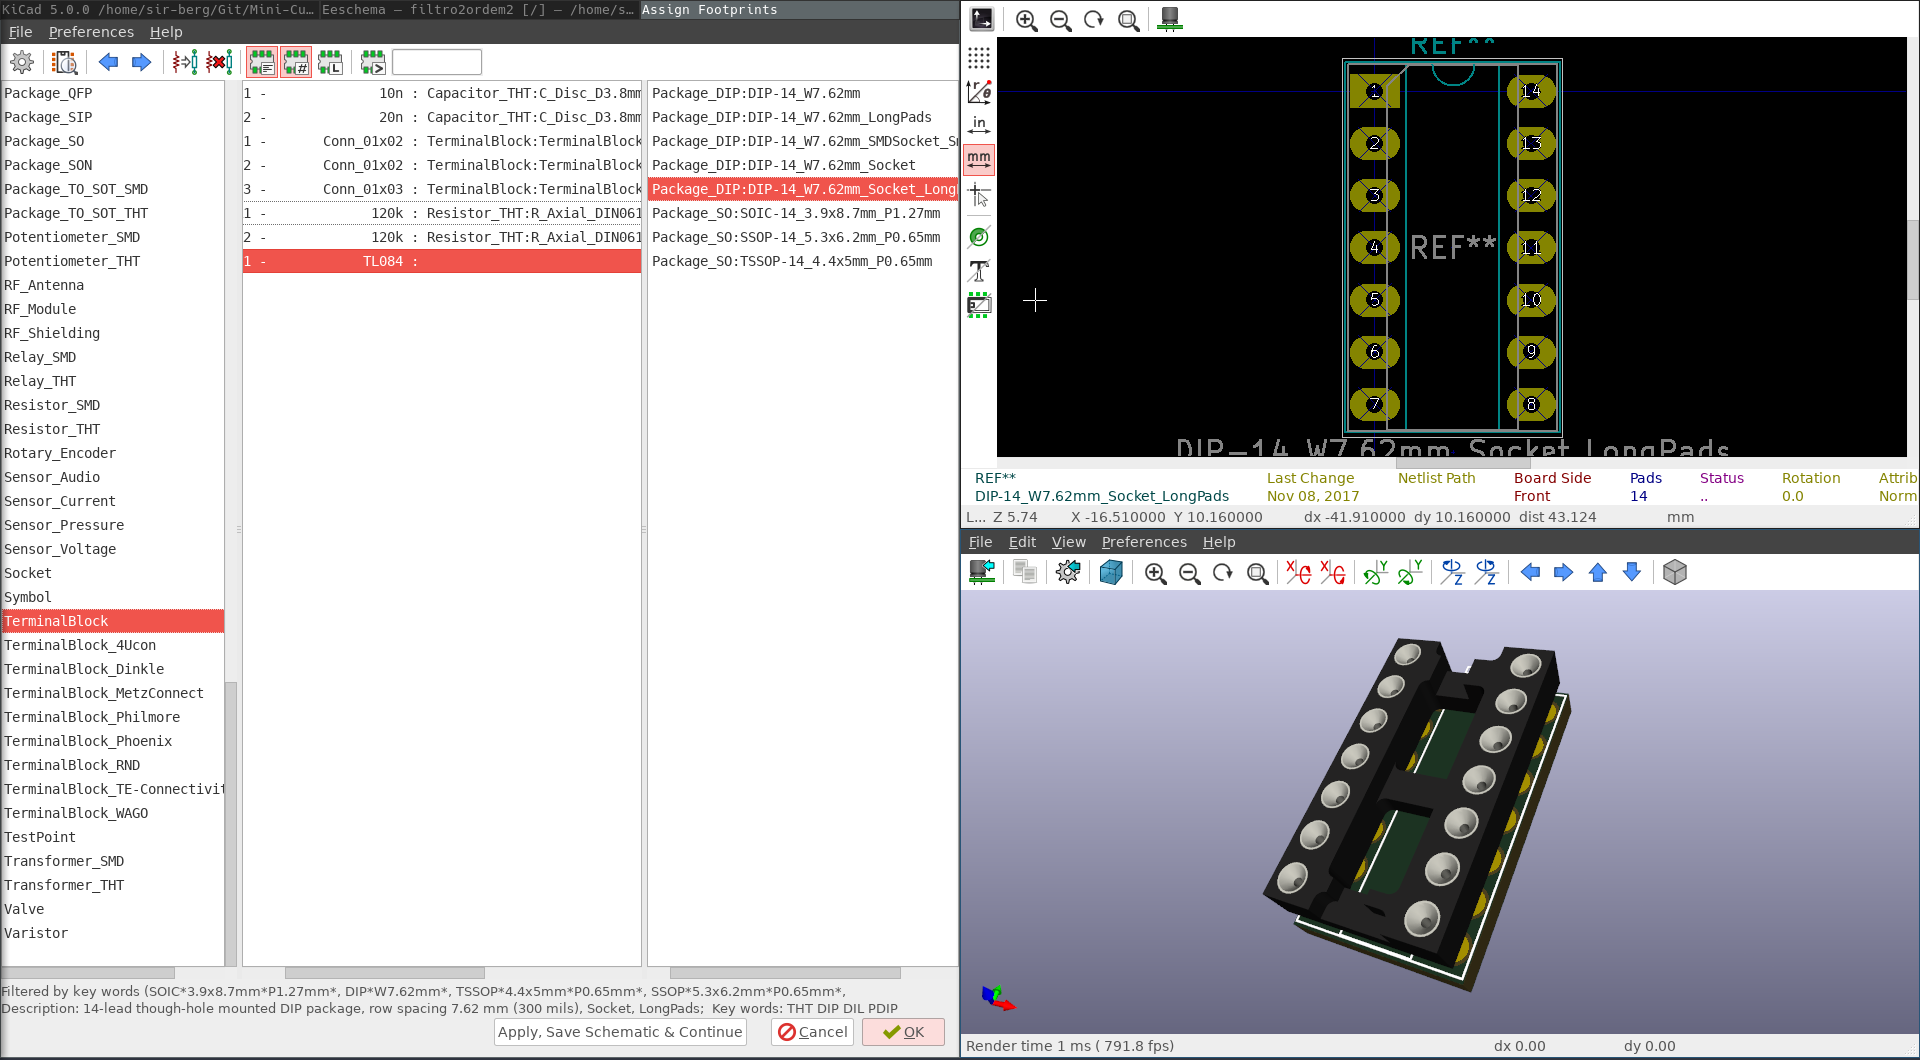
\includegraphics[width=0.65\textwidth]{Imagens/23_terminando_associar.png}
		\caption{Terminando de associar os componentes}
	\end{figure}
	\pause
	\begin{itemize}
		\item \texttt{Crtl+s} para salvar.
		\item Gerar novamente o \textit{netlist} para agora ele ser atualizado com os componentes já associados.
	\end{itemize}
\end{frame}

\section{Fazendo roteamento da PCB.}
\begin{frame}{Entrando no modo PCB}
	\begin{figure}
		\centering
		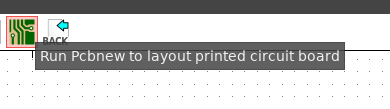
\includegraphics[width=0.7\textwidth]{Imagens/24_rodando_pcbnew.png}
		\caption{Opção no menu superior da janela de esquemático para entrar no modo PCB.}
	\end{figure}
\end{frame}

\begin{frame}{No modo PCB}
	\begin{block}{O que fazer?}
		\begin{itemize}
			\item Carregar o \textit{netlist} gerando anteriormente.
			\item Atribuir padrão de projeto.
			\item Rotear as placas.
			\item Adicionar malha de terra.
		\end{itemize}
	\end{block}
		\pause
	\begin{figure}
		\centering
		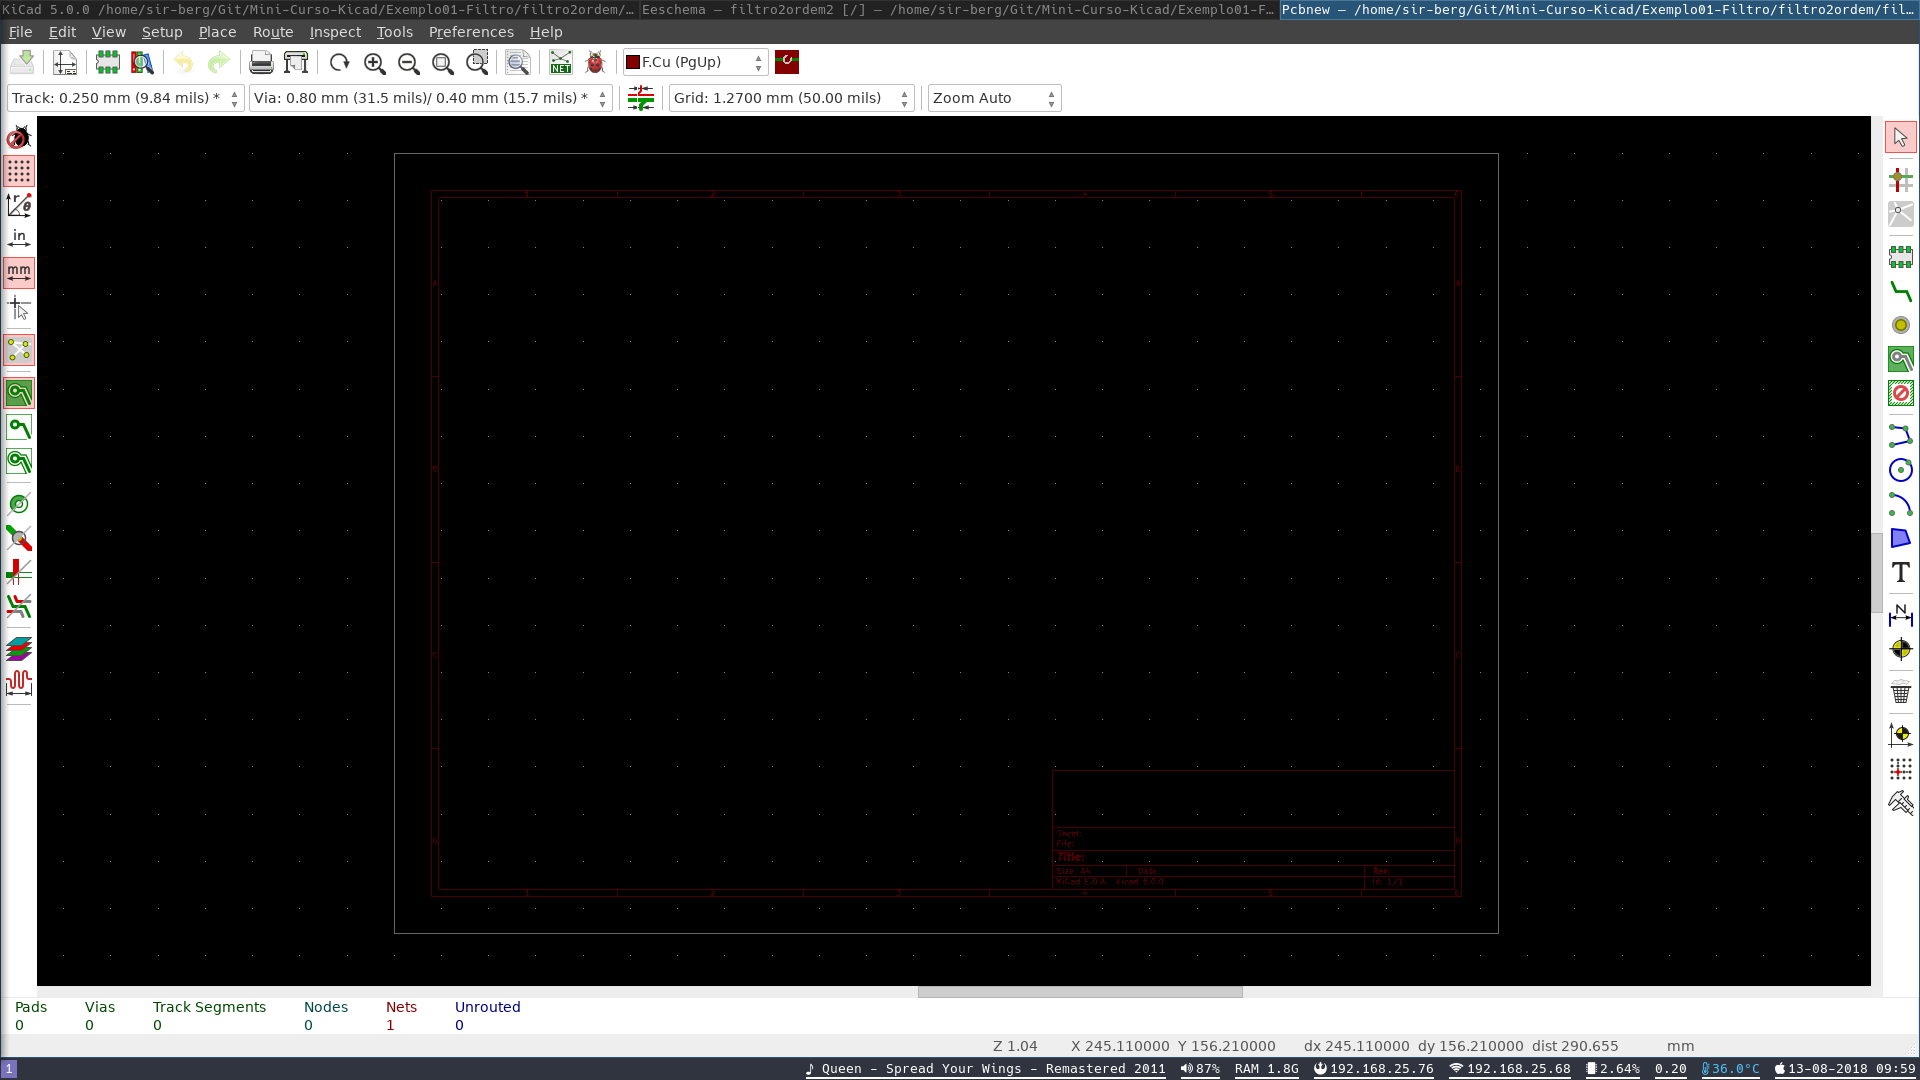
\includegraphics[width=0.65\textwidth]{Imagens/25_janela_pcbnew.png}
		\caption{Janela do PCB \textit{new}.}
	\end{figure}
\end{frame}

\begin{frame}{Lendo o \textit{Netlist}}
	\begin{block}{Por que?}
		\begin{itemize}
			\item O \textit{netlist} tem a descrição do circuito e dos componentes que serão roteados na PCB.
		\end{itemize}
	\end{block}
	\begin{figure}
		\centering
		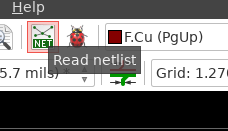
\includegraphics[width=0.7\textwidth]{Imagens/26_read_netlist.png}
		\caption{Localização no menu superior para ler o \textit{netlist}.}
	\end{figure}
\end{frame}

\begin{frame}{Lendo o \textit{Netlist}}
	\begin{itemize}
		\item Para ler o \textit{netlist} gerado anteriormente basta selecionar a localização do \textit{netlist} e ler ele.
		\item A leitura deu certo quando aparece as escritas verdes na saída de log e quando aparece os componentes da janela do PCB \textit{new}.
	\end{itemize}
	\begin{figure}
		\centering
		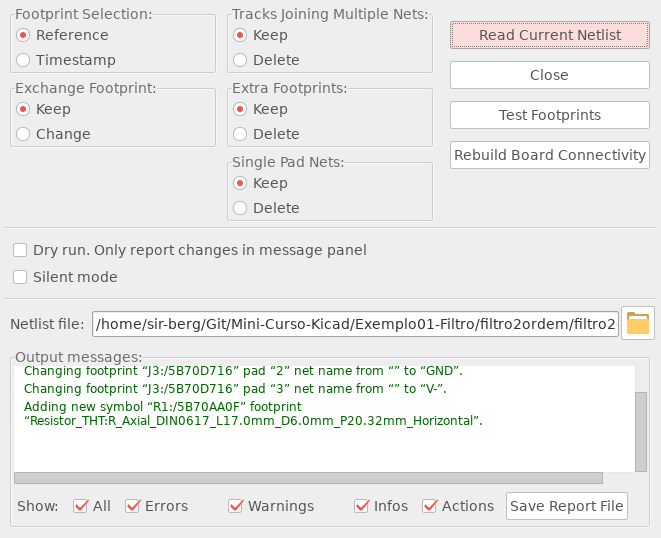
\includegraphics[width=0.4\textwidth]{Imagens/27_read_netlist_janela.png}
		\caption{Janela para leitura do \textit{netlist}.}
	\end{figure}
\end{frame}

\begin{frame}{Após leitura do \textit{netlist}}
	\begin{figure}
		\centering
		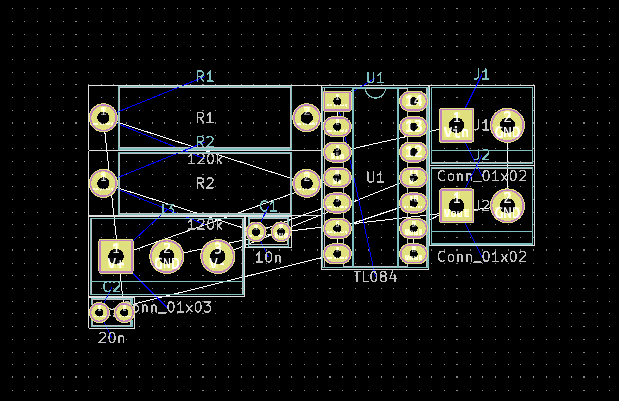
\includegraphics[width=0.7\textwidth]{Imagens/28_componentes_board.png}
		\caption{Componentes na área de trabalho do PCB \textit{new}.}
	\end{figure}
	\pause
	\begin{itemize}
		\item Agora é só rotear a placa, mas antes é preciso definir uma regra de design.
	\end{itemize}
\end{frame}

\begin{frame}{\textit{Design Rules}}
	\begin{block}{Pra que serve?}
		\begin{itemize}
			\item Definir padrões para as trilhas e suas medidas, a fim de que não seja criada PCBs com trilhas frágeis.
		\end{itemize}
	\end{block}
	\begin{figure}
		\centering
		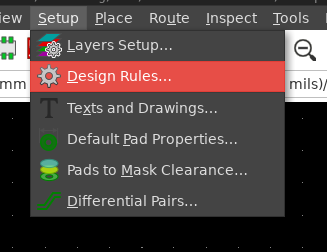
\includegraphics[width=0.45\textwidth]{Imagens/30_design_rules.png}
		\caption{Local no menu superior para acessar a opção das regras de design.}
	\end{figure}
\end{frame}

\begin{frame}{\textit{Design Rules}}
	\begin{figure}
		\centering
		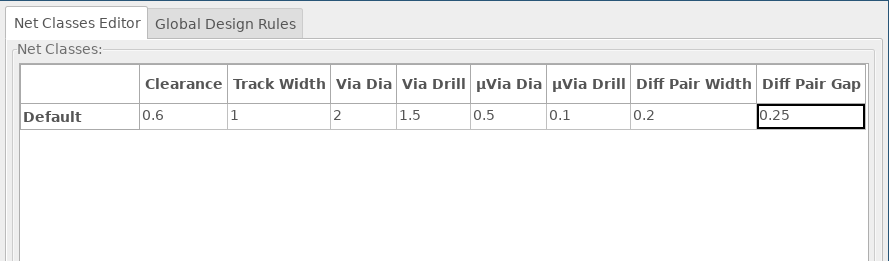
\includegraphics[width=1\textwidth]{Imagens/31_design_padrao.png}
		\caption{Janela da opção para mudar as regras de design.}
	\end{figure}
\end{frame}

\begin{frame}{Design Rules}
	\begin{itemize}
		\item \textit{Clearance} - Distância entre a trilha e uma linha que limita a trilha mais próxima dela.
		\item \textit{Track width} - Largura da trilha.
	\end{itemize}
	\begin{figure}
		\centering
		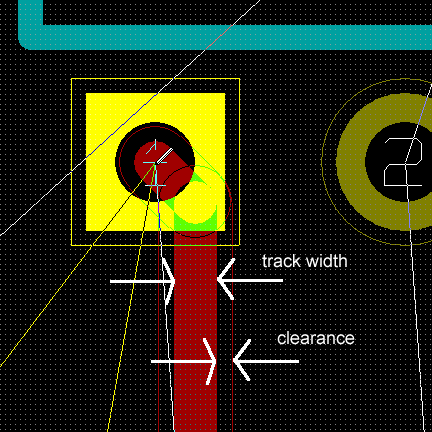
\includegraphics[width=0.4\textwidth]{Imagens/30_clearance.png}
		\caption{Diferença entre \textit{clearance} e \textit{track width}(largura da trilha).}
	\end{figure}
\end{frame} 

\begin{frame}{Atalhos do modo PCB}
	\begin{block}{Atalho com o componente ou trilha selecionado}
		\begin{itemize}
			\item \texttt{X} - Trilhas.
			\item \texttt{M} - Mover componente.
			\item \texttt{R} - Rotacionar.
		\end{itemize}
	\end{block}
\end{frame}

\begin{frame}{Organizando o circuito para rotear as trilhas}
	\begin{figure}
		\centering
		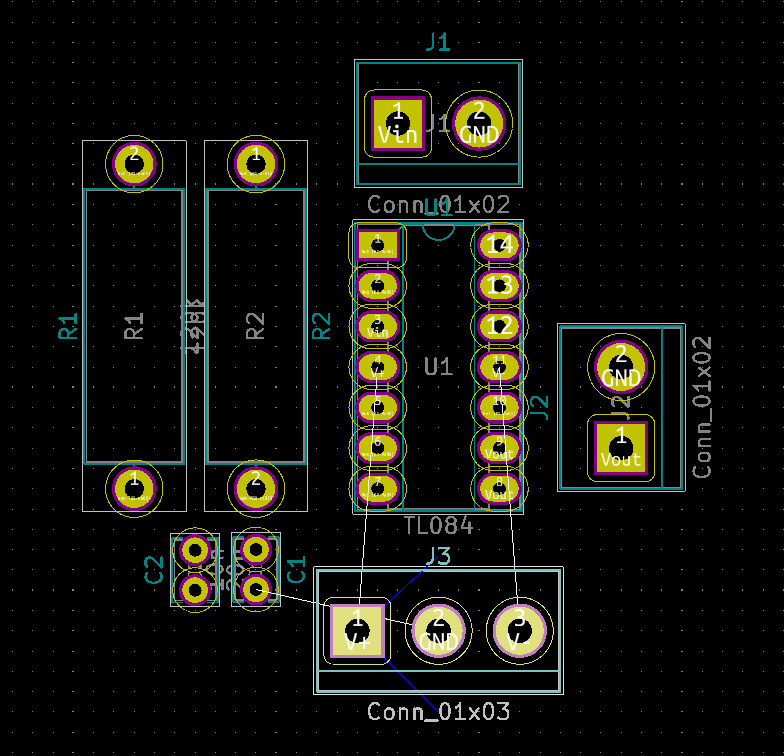
\includegraphics[width=0.6\textwidth]{Imagens/32_organizacao_circuito.png}
		\caption{Organização do circuito.}
	\end{figure}
\end{frame}

\begin{frame}{\textit{Layers}}
	\begin{block}{Escolhendo}
		\begin{itemize}
			\item Sempre a \textit{background}.
			\item A \textit{layer forenground} é para caso de placas dupla face.
			\item Geralmente só se usa a \textit{background}.
		\end{itemize}
	\end{block}
	\begin{figure}
		\centering
		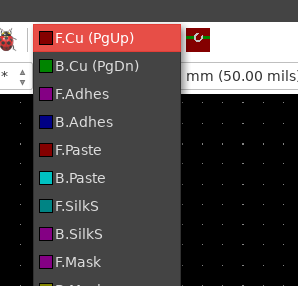
\includegraphics[width=0.35\textwidth]{Imagens/33_layers.png}
		\caption{Menu para selecionar as \textit{layers}.}
	\end{figure}
\end{frame}

\begin{frame}{Filtro pré-roteado}
	\begin{figure}
		\centering
		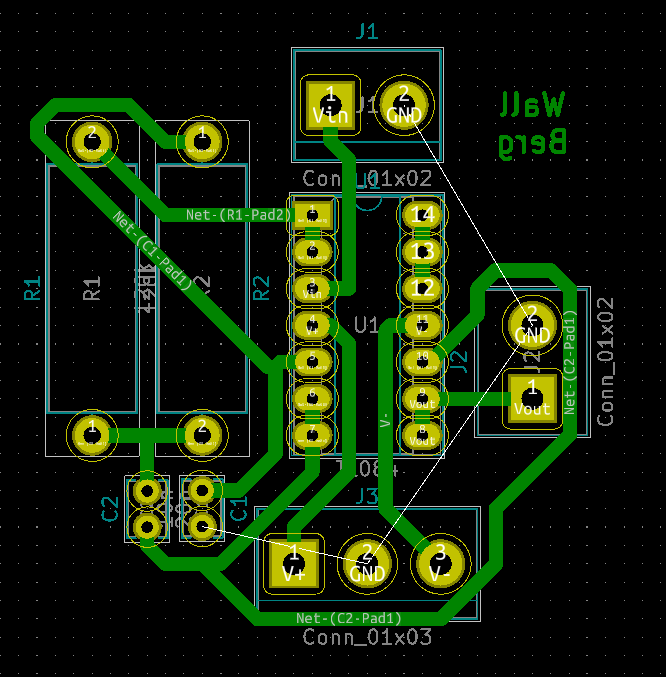
\includegraphics[width=0.5\textwidth]{Imagens/34_circuito_pre_router.png}
		\caption{Circuito pré-roteado}
	\end{figure}
\end{frame}

\begin{frame}{Adicionando malha de terra}
	\begin{block}{Pra que serve?}
		\begin{itemize}
			\item Reza a lenda que é pra eliminar ruído na placa.
		\end{itemize}
	\end{block}
	\begin{figure}
		\centering
		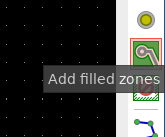
\includegraphics[width=0.5\textwidth]{Imagens/35_add_malha_terra.png}
		\caption{Opção no menu do lado direito do PCB \textit{new}.}
	\end{figure}
\end{frame}

\begin{frame}{Adicionando malha de terra}
	\begin{block}{Selecionando o ponto de terra}
		\begin{itemize}
			\item É preciso selecionar o pino que será utilizado como um ponto em comum na placa.
		\end{itemize}
	\end{block}
	\begin{figure}
		\centering
		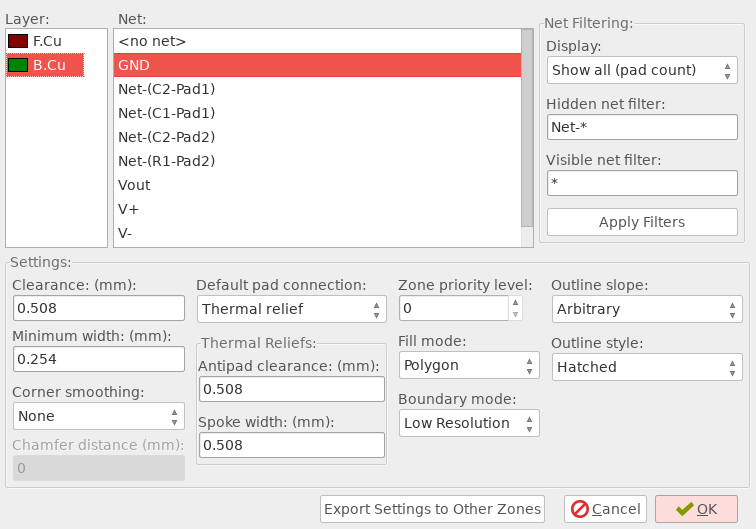
\includegraphics[width=0.55\textwidth]{Imagens/36_malha_terra_janela.png}
		\caption{Janela com opções de malha de terra.}
	\end{figure}
\end{frame}

\begin{frame}{Circuito com malha de terra}
	\begin{figure}
		\centering
		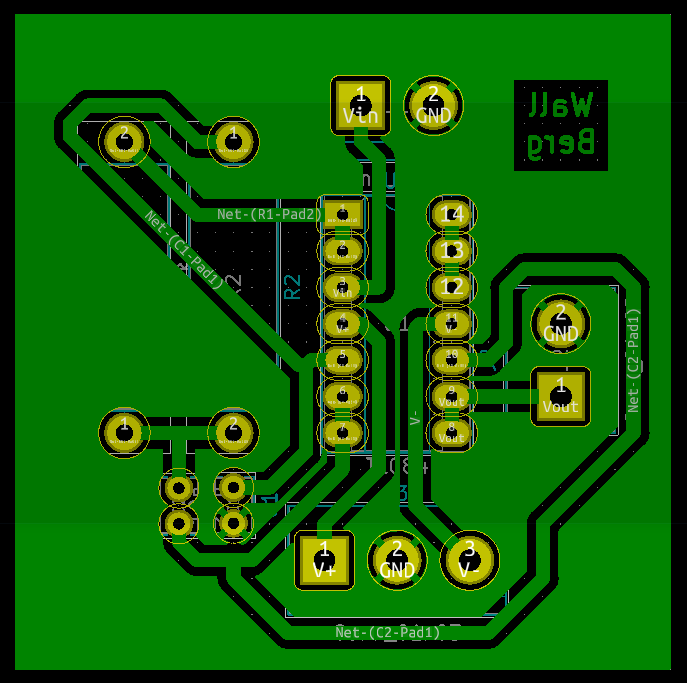
\includegraphics[width=0.5\textwidth]{Imagens/37_circ_com_malha.png}
		\caption{Circuito com malha de terra}
	\end{figure}
\end{frame}

\begin{frame}{Quando a placa está pronta??}
	\begin{itemize}
		\item Somente quanto a placa não tiver mais pinos sem conectar.
	\end{itemize}
	\begin{figure}
		\centering
		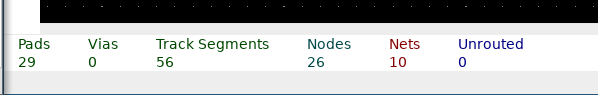
\includegraphics[width=1\textwidth]{Imagens/38_0_unrouted.png}
		\caption{PCB sem pinos para conectar.}
	\end{figure}
\end{frame}

\begin{frame}{Visualização 3D da placa}
	\begin{figure}
		\centering
		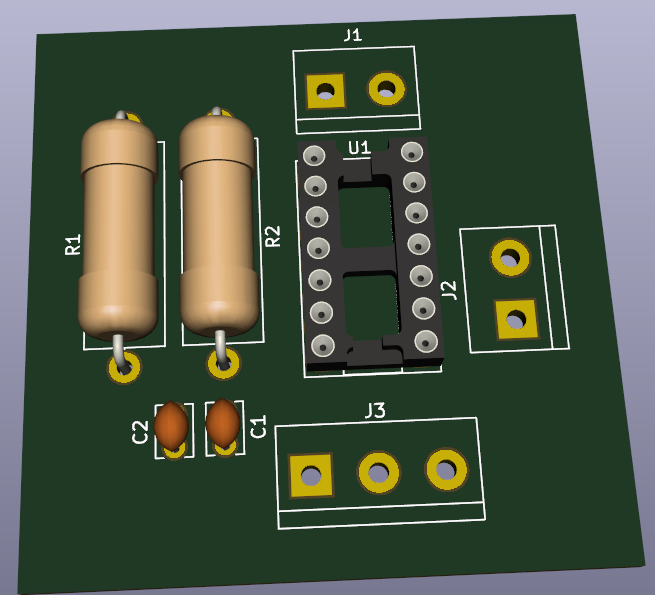
\includegraphics[width=0.6\textwidth]{Imagens/40_3d_view.png}
		\caption{Visualização 3D vista de cima.}
	\end{figure}
\end{frame}

\begin{frame}{Visualização 3D da placa}
	\begin{figure}
		\centering
		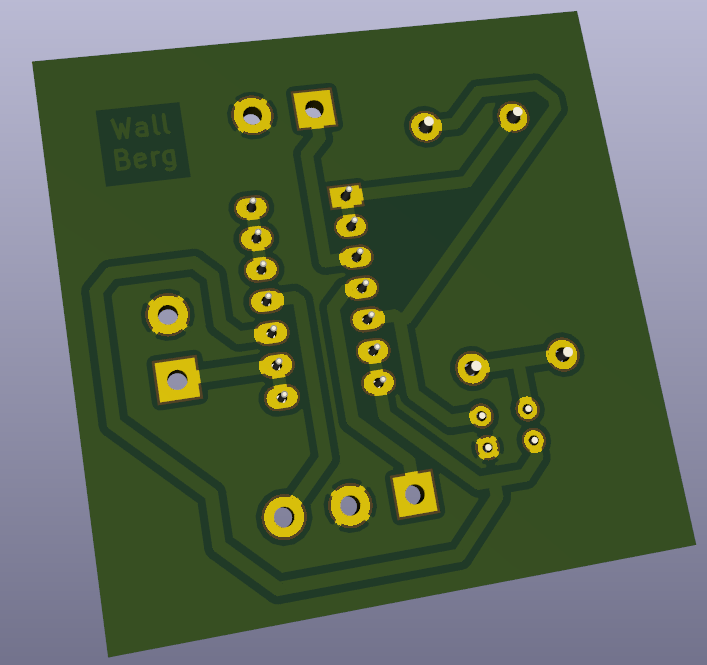
\includegraphics[width=0.6\textwidth]{Imagens/40_3d_view_2.png}
		\caption{Visualização 3D vista de baixo.}
	\end{figure}
\end{frame}

\section{Imprimindo o \textit{layout} da PCB}
\begin{frame}{Imprimindo o \textit{layout} da PCB}
	\begin{block}{O que precisa?}
		\begin{itemize}
			\item Papel fotográfico.
		\end{itemize}
	\end{block}
	\begin{block}{Antes de imprimir}
		\begin{itemize}
			\item Duplique sua placa para caso perder um pedaço, tem outro de reserva.
		\end{itemize}
	\end{block}
\end{frame}

\begin{frame}{Imprimindo o \textit{layout} da PCB}
	\begin{block}{Atalho}
		\begin{itemize}
			\item \texttt{Ctrl+D} - Duplicar área selecionada.
		\end{itemize}
	\end{block}
	\begin{figure}
		\centering
		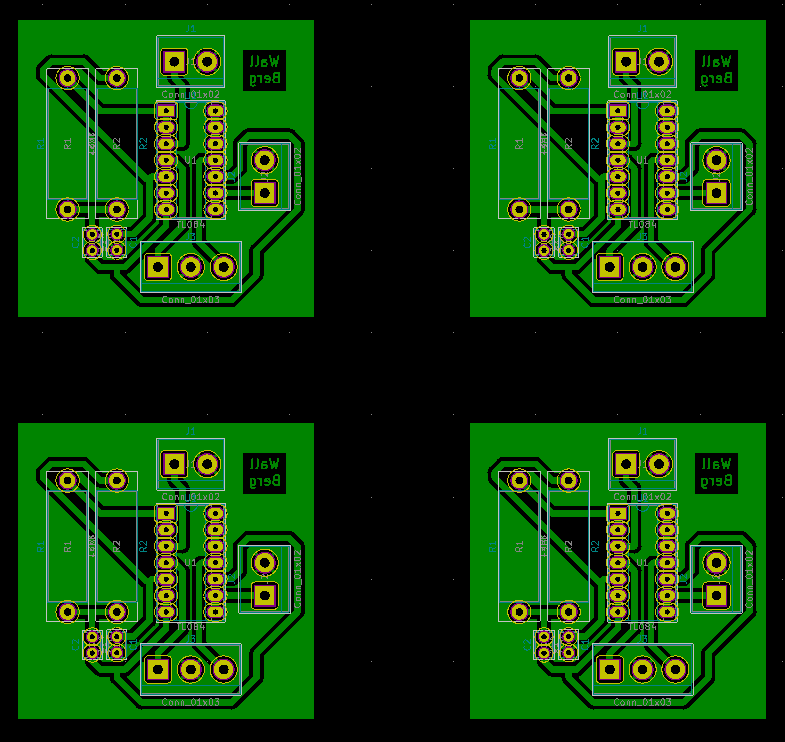
\includegraphics[width=0.45\textwidth]{Imagens/39_duplicate.png}
		\caption{\textit{Layout} duplicado.}
	\end{figure}
\end{frame}

\begin{frame}{Imprimindo o \textit{layout} da PCB}
	\begin{figure}
		\centering
		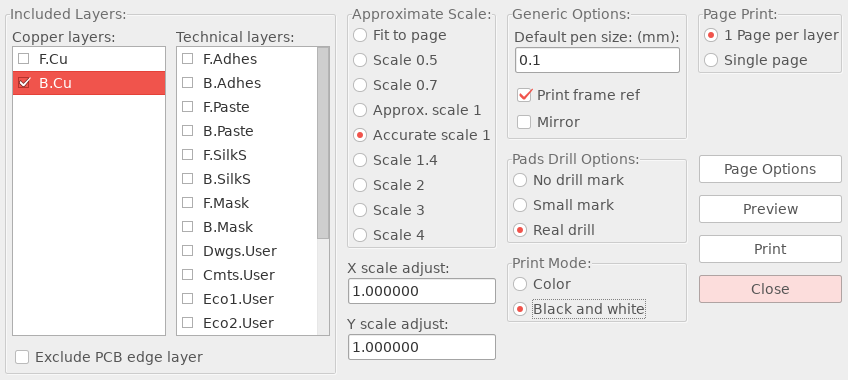
\includegraphics[width=1\textwidth]{Imagens/41_print_janela.png}
		\caption{Janela com opções de impressão de PCB.}
	\end{figure}
\end{frame}

\begin{frame}{Imprimindo o \textit{layout} da PCB}
	\begin{figure}
		\centering
		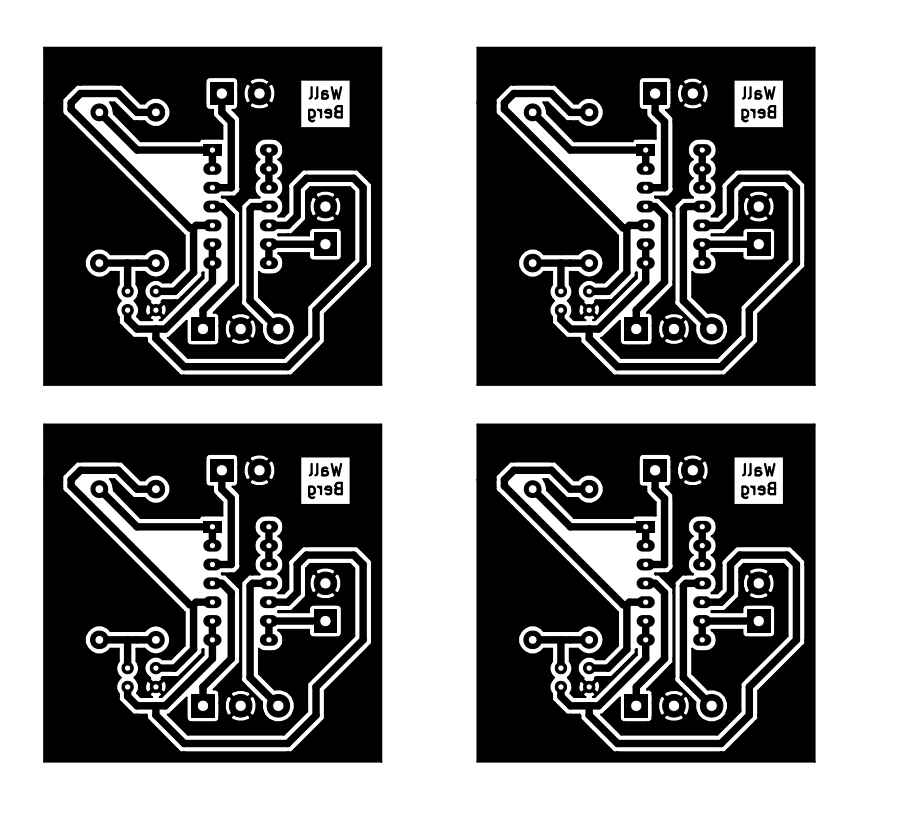
\includegraphics[width=0.6\textwidth]{Imagens/42_placa_final.png}
		\caption{Placa final que será impresso no papel fotográfico.}
	\end{figure}
\end{frame}

\begin{frame}{Agradecimentos}
	\begin{itemize}
		\item Muitíssimo obrigado pela atenção de todos.
		\item Agradeço ao CA pela oportunidade de ministrar esse minicurso.
	\end{itemize}
\end{frame}

\begin{frame}
	\titlepage
\end{frame}

\end{document}